\chapter{Design}


This chapter go through the design steps that are taken in each stage of the research. Initially this research is started as\textbf{ Compile time server architectures for Ballerina}. After several evaluations with the result in stage, focus area is narrowed down to finding optimal thread pool size based on programming features. Machine learning approach is used to predict thread pool size. Research questions remain unchanged from the beginning since thread pools are crucial part in web server architectures. The initial idea was to maximize performance of each use case ( program) by tuning or implementing new server architectures in Ballerina run time. Literature review indicates that performance of single web server architecture differ according to type of workload (use case) it execute. In simple terms different web server architecture perform differently for different user application. Tuning server architectures able to maximize the performance for some use cases.

Formal research methodology is based on Design science \cite{design_science} approach. Design science research requires the creation of an innovative, purposeful artifact for a special problem domain. The artifact must be evaluated in order to ensure its utility for the specified problem. In order to form a novel research contribution, the artifact must either solve a problem that has not yet been solved, or provide a more effective solution. Both the construction and evaluation of the artifact must be done rigorously, and the results of the research presented effectively both to technology-oriented and management-oriented audiences.

This research tries to provide more effective solutions to a current problem and creates innovative solutions by introducing techniques to predict optimal thread pool size based on program features.

%\section{Problem investigation}
%
%Investigation of the problem requires comprehensive literature review on server architectures and how well current web server architectures performed on different workloads. It also needs to show that well tuned architectures perform better than the original implementation. In next phases it requires to identify what are the performance critical features that affect the performance of server architectures. Then it is required to build a model to predict optimal tune (size of the thread pool) of the server architecture 


\section{Moving in to research}

In this research we try to resolve one conclusion made from a previous study \cite{comp_ac} which is to automatically and dynamically tune the web server architecture to efficiently execute the offered workload. In all the previous studies, differentiating the workload is done by user. This study proposes a technique to identify workload at compile time of the program and predict the optimal server architecture ( thread pool size) using machine learning approach. 

This research is consist of following areas. Next section will explain the steps taken to answer the research question mentioned in chapter 1.

\begin{enumerate}
	\item Evaluate performance of different web server architectures and fine tune them.
	\item Identify features in Ballerina programs that affect the performance of server architecture.
\end{enumerate}

In order to understand the design steps it is important to specify internal architecture of Ballerina run time. Next section briefly explain the internals of the Ballerina.

\section{Ballerina}\label{Sec_Ballerina}

As growing needs of the distributed computing rapid development of web services, new programming languages and paradigms were invented. Ballerina \cite{ballerina} is such a successful language that handles network programming in a developer friendly way. Following quotes a small paragraph from the ballerina official website.


\say{For decades, programming languages have treated networks simply as I/O sources. Ballerina introduces fundamental, new abstractions of client objects, services, resource functions, and listeners to bring networking into the language so that programmers can directly address the Fallacies [20] of Distributed Computing as part of their application logic. This facilitates resilient, secure, performant network applications to be within every programmer’s reach.}


Also Ballerina programming language has certain capabilities extracting programming features, especially IO calls. In ballerina they are called connector calls. Thus extracting features that affect the performance is easier as network calls are first class citizens in Ballerina languages. In the source code they are explicitly stating as “ - $>$“. Then it is able to extract such features statically from the \acrfull{AST} of the ballerina source code.


Following is one example how the database calls are represented in ballerina code, note the -$>$ symbol.\\

\textit{stream$<$record{}, error$>$ resultStream = mysqlClient4 - $>$ query(<@untainted>query);}\\


Other languages provide network operations as library functions.If we try to extract such features from other languages we need to know exactly this function call to do an IO operation. That is an impossible task to extract such features just exploring the source code in other languages like C,Java etc.


It is clear that we can use the network awareness properties  of the Ballerina language to identify performance critical features directly from source code unlike other languages. Examples of network awareness features are creating RESTful clients and servers, making database queries, completing asynchronous calls, producing and consuming streaming data message-passing etc \cite{ballerina_book}.

Also network services are first order objects in ballerina language like functions \cite{ballerina_book}. Such features can be used to identify whether a given program is a network service or not. In other languages we need to have prior knowledge about which libraries are used for such implementations.


\subsection{Ballerina internal architecture}

This section explains the main components of Ballerina run time.

\subsubsection{Scheduler}

Ballerina scheduler is the main component for every program which runs. The Ballerina scheduler executes the workload using it’s own thread pool. The default thread pool size is two times the available processor count of the operating system. All the tasks which need to executed are held in a queue. Then threads in the thread pool access the queue and execute the task. This is where major turnings are happen at final stage of the research. 

\subsubsection{Netty Layer}

This layer is implemented using a library called Netty \cite{netty}. Primary task of the Netty layer is to listen for Http client connections and manage the session. It has its own thread pools to handle those connections. In original ballerina architecture this layer simply handed over the incoming connection to the ballerina scheduler. Then the scheduler invokes the relevant tasks for the client and returns the results to the Netty layer again for submitting back to the client.

\subsubsection{Resource function}

In ballerina each API endpoint can be implemented as a resource function. That function includes all the implementation required to fulfill the task that client is requested. More details about resource function is stated in Chapter 4. In this research each resource functions are considered as programs.


Figure \ref{bal_internal} shows high level view of Ballerina architecture.


\begin{figure}[htbp]
	\begin{center}
		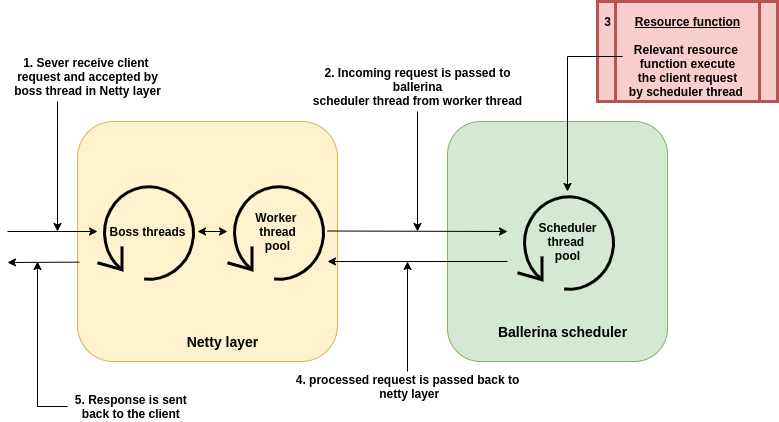
\includegraphics[scale=0.5]{figures/bal-internal.png}
	\end{center}
	\caption{Ballerina's internal architecture}
	\label{bal_internal}
\end{figure}

\section{Design steps}

The initial idea is coupled with bound type of the program (CPU bound and IO bound). Targets were, (1) for a given Ballerina program identify its bound type, then (2) switch the server architecture which best suits the bound type. To determine the best  server architecture experiments are conducted. Following steps are taken to conduct the experiments. Below process is iterative.

\begin{itemize}
	\item Implement server architectures
	\item Implement benchmark programs which have CPU intensive task and IO intensive tasks
	\item Analyze results
	\item Introduce more tunes to architecture based on previous results
\end{itemize} 

\subsection{Testing process}

Each testing program is hosted as HTTP endpoints. Calling that endpoint invokes the relevant program. Jmeter act as a HTTP client. Typical web server able to process concurrent HTTP requests. Jmeter can be configured to model this behavior. Jmeter continuously calls the given endpoint for certain period under given configurations such as concurrency level. Then the following metrics are recorded,

\begin{itemize}
	\item Average latency
	\item Stranded deviation of latency
	\item Throughput (Request per second)
	\item Error rate
	\item Median, 75th percentile, 99th percentile of latency
\end{itemize} 

Then the performance are evaluated using above metrics. As an example when average latency is low and throughput is high for given endpoint, that architecture is good for the relevant use case. 
  

\begin{figure}[htbp]
	\begin{center}
		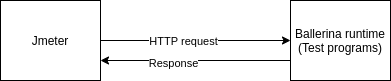
\includegraphics[scale=0.5]{figures/jmeter_bal.png}
	\end{center}
	\caption{Jmeter and Ballerina run time}
	\label{jmeter_testing}
\end{figure}



\subsection{Phase I - Implement and evaluate performance of different server architectures}

In this phase following server architectures are implemented. 

 \begin{itemize}
 	\item Original Ballerina architecture
 	\item Netty OIO
 	\item Removing Ballerina scheduler thread pool
 	\item Tuning Ballerina scheduler thread pool size
 \end{itemize} 

Original Ballerina architecture mainly consist of two thread pools. One thread pool belongs to Ballerina scheduler and other thread pool belongs to Netty layer. Fine tuning and implementing new architecture involves changing the behavior of these thread pools. In Netty OIO , worker thread pool is converted to have blocking IO. Then each connection spawn a new thread. Originally these thread pools has non-blocking behavior. Next architectural change is removing the Ballerina scheduler thread pool. \textbf{Default thread pool size of Ballerina scheduler} is \textbf{$ \boldsymbol{2} \times \boldsymbol{Number\: of\: CPU\: cores}$}. Then the workload is executed by Netty threads. 

After conducting experiments with above architectures, following conclusions were made,
 
\begin{itemize}
	\item Netty OIO performance is worse in every situation - thus this architecture was no longer considered
	\item Removing Ballerina scheduler perform well in every situations
\end{itemize} 

Results are discussed in Chapter 5. Based on these results experiments were conducted with changing size of the thread pool in Ballerina scheduler.

\subsubsection{Test programs}

Following programs were implemented to evaluate the performance of each architectural change,

  \begin{itemize}
  	\item Check whether given number is prime - 3 primes are checked as small (521),medium(7919) and large(1000003)
  	\item Merge sort - 1000 random numbers are sorted
  	\item Read File from disk
  	\item ‘select’ query on mysql database
  \end{itemize} 
Above programs cover the CPU intensive cases and IO intensive cases. 

Sample representation of single experiment is shown in figure \ref{sample_result}. Four metrics (throughput, slandered divination, mean - average latency, 99th percentile  ) are shown in the plot. X-axis represents the concurrent users. Y-axis represents the  relevant metric. 

 \begin{figure}[htbp]
 	\begin{center}
 		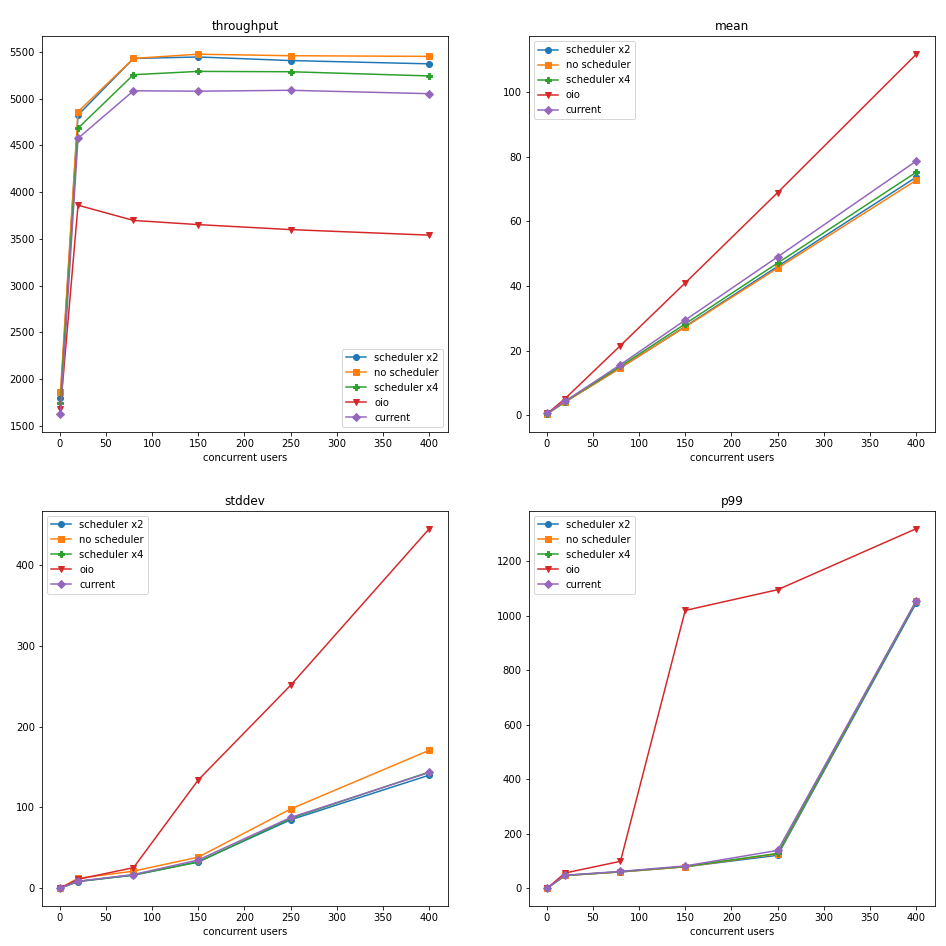
\includegraphics[scale=0.35]{figures/prime_small test results.png}
 	\end{center}
 	\caption{Sample experiment result}
 	\label{sample_result}
 \end{figure}

In this phase goal was to obtain metric similar to table \ref{tab:result_metric}. \textbf{Pool size x 2} and \textbf{Pool size x 4} represent the multiplier of original thread pool size in Ballerina scheduler which is \textbf{$ \boldsymbol{2} \times \boldsymbol{Number\: of\: CPU\: cores}$}. As an instance if the environment have 2 CPU cores,  \textbf{Pool size x 2} indicate 4 threads.


\begin{table}[]
	\begin{center}
	\begin{tabular}{|l|l|l|l|l|l|}
		\hline
		Test case                                                     & \multicolumn{5}{l|}{Server architecture}                                                                                                                                                                                                                                \\ \hline
		& \begin{tabular}[c]{@{}l@{}}Ballerina \\ original\end{tabular} & \begin{tabular}[c]{@{}l@{}}No \\ scheduler\end{tabular} & Netty OIO & \begin{tabular}[c]{@{}l@{}}Thread pool\\  size x 2\end{tabular} & \begin{tabular}[c]{@{}l@{}}Thread pool\\  size x 4\end{tabular} \\ \hline
		\begin{tabular}[c]{@{}l@{}}Prime check \\ small\end{tabular}  &                                                               &                                                         &           &                                                                 &                                                                 \\ \hline
		\begin{tabular}[c]{@{}l@{}}Prime check \\ medium\end{tabular} &                                                               &                                                         &           &                                                                 &                                                                 \\ \hline
		\begin{tabular}[c]{@{}l@{}}Prime check \\ large\end{tabular}  &                                                               &                                                         &           &                                                                 &                                                                 \\ \hline
		\begin{tabular}[c]{@{}l@{}}Database \\ call (IO)\end{tabular} &                                                               &                                                         &           &                                                                 &                                                                 \\ \hline
		Merger sort                                                   &                                                               &                                                         &           &                                                                 &                                                                 \\ \hline
		File read                                                     &                                                               &                                                         &           &                                                                 &                                                                 \\ \hline
	\end{tabular}
	\end{center}
	\caption{Architecture comparison metric}
	\label{tab:result_metric}
\end{table}


After few iterations of this phase, no architecture performed well for IO use cases rather CPU intensive cases and vice versa. Changing architecture either performed worse or well for all the use cases. Although changing thread pool size in Ballerina scheduler started to show some significance result. Increasing thread pool size was affected differently in IO use cases. Then the Design phase 2 was continued with varying the thread pool size in Ballerina original architecture.

\subsection{Phase II - Tuning thread pool size}

Tuning thread pool size can be approached in two ways, \textbf{(1) White box system} - This requires complex mathematical modeling with queuing theories \cite{math_aproach_thread_pool_tuning}. Initial approach is cannot be archived with this model which is predicted optimal web server architecture based on programming features. \textbf{(2) Black box system} - In this approach thread pool system is considered as a black box, then experiments are run with thread pool size changes. Figure \ref{black_box_boundary} shows boundary of the black box.

 
\begin{figure}[htbp]
	\begin{center}
		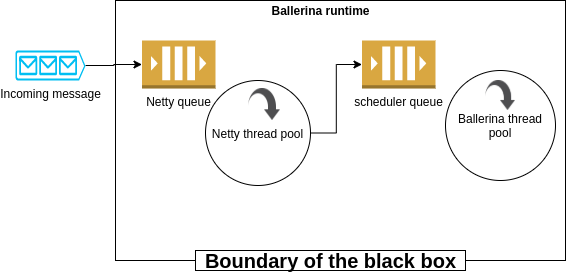
\includegraphics[scale=0.5]{figures/black_box_boundary.png}
	\end{center}
	\caption{Boundary of the black box}
	\label{black_box_boundary}
\end{figure}


This phase is proceeded considering the system as black box. This model allows executing different programs under different size of thread pool. These programs consist of CPU intensive operations, IO intensive operations and mixed operations where both IO and CPU intensive operations exist. To proceed the experiments fixed concurrency level (Number of concurrent clients) is selected. 
Limitation of this approach are,

\begin{itemize}
	\item Results are dependent on selected concurrency level
	\item Results are dependent on selected environment (Eg: Number of CPU)
	
\end{itemize} 
More experiments are required to generalize this approach to other environments and various concurrency levels. Due to limitation of time period, this level is not discussed in the research. 
	
\subsubsection{Experimental design} 

Number of new programs were implemented to conduct the experiments. As a primary metric of evaluation average latency is used. Various programs are designed referring multiple sources. The aim is make these programs to close real world applications. Extracting features of these programs are discussed in Design phase III. Then each program is run under different thread pool sizes. Then metrics are recorded. Table \ref{tab:pool_size_latency} shows summery of the results. Empty cells represent the average latency. Minimum latency value provide the optimal thread pool size for given program. 

\begin{table}[]
	\begin{center}
	\begin{tabular}{|l|l|l|l|l|l|l|}
		\hline
		Program    & \multicolumn{6}{l|}{Pool size}        \\ \hline
		& 1            & 2 & 3 & ... & 19 & ... \\ \hline
		Program 1  & Ave. latency &   &   &     &    &     \\ \hline
		Program 2  &              &   &   &     &    &     \\ \hline
		Program 3  &              &   &   &     &    &     \\ \hline
		...        &              &   &   &     &    &     \\ \hline
		Program 50 &              &   &   &     &    &     \\ \hline
		...        &              &   &   &     &    &     \\ \hline
	\end{tabular}
	\end{center}
	\caption{Program vs. Thread pool size - Latency results}
	\label{tab:pool_size_latency}
\end{table}

\subsection{Phase III - Building machine learning model to predict optimal thread pool size for given program}

At first two models are considered addition to predicting optimal thread pool. One model directly predict the latency with given program features and given thread pool size. This model can be expressed as following function. 

$$ Latency \:(ms) = f(\:Program\:features,\:Threadpool\:size\:)$$

Weakness of this model is it heavily depend on nature of IO call. As an example latency is dependent on where the database is hosted if the given program has database call. Also, latency is affected by the network connection also. Then the generalization of result is very difficult.

The next model predict optimal thread pool size for the given program. That model can be expressed as follows.

$$ Optimal\:thread\:pool\:size = f(\:Program\:features)$$

In order to build this model it is required find the minimum thread pool value from the result obtained by Design phase II. This step can be abstracted as in figure \ref{optimal_pool_size}

\begin{figure}[htbp]
	\begin{center}
		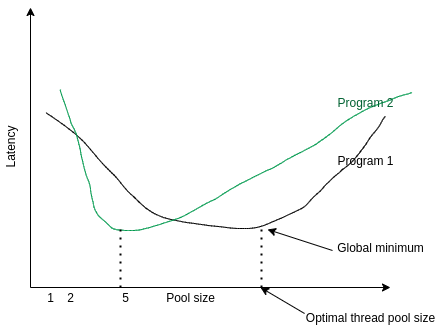
\includegraphics[scale=0.5]{figures/optimal_pool_size.png}
	\end{center}
	\caption{Obtaining optimal thread pool size}
	\label{optimal_pool_size}
\end{figure}

After some feature engineering steps following features are selected to train the machine learning model.

 \begin{itemize}
 	\item Number of HTTP connector calls
 	\item Number of Database connector calls
 	\item Number of non-blocking gRPC convector calls
 	\item Whether each type of connector calls lies inside a loop 
 	\item Whether loops are present
 	\item More features to analyze ...
 \end{itemize} 

Then a training data set is created where input features are above programming features and output is optimal thread pool size. Table \ref{tab:data_frame} shows the shape of the data frame.


	\begin{table}[]
		\begin{center}
		\begin{tabular}{|l|l|l|l|l|l|}
			\hline
			\multirow{2}{*}{Program} & \multicolumn{4}{l|}{Features} & \begin{tabular}[c]{@{}l@{}}Thread pool\\  size\end{tabular} \\ \cline{2-6} 
			& F 1    & F2    & ..    & Fn   &                                                             \\ \hline
			Program 1                &        &       &       &      &                                                             \\ \hline
			...                      &        &       &       &      &                                                             \\ \hline
		\end{tabular}
	\end{center}
		\caption{Data frame shape}
		\label{tab:data_frame}
	\end{table}

Then following machine learning models are selected and evaluated the accuracy of each model.

\begin{itemize}
	
	\item XGBoost
	\item Support Vector Machine
	\item Decision Tree
	\item Random Forest
	
\end{itemize}

For regression models \acrfull{MAPE} and \acrfull{MSE} are evaluated. For classification models F1 score and accuracy are evaluated.

\textbf{...Incomplete..}

\begin{itemize}
	
	\item How classification model is built
	\item Why regression
	
\end{itemize}


\subsection{Phase IV - Parsing Ballerina AST to obtain features}

In this phase a module is designed to parse Ballerina source code to feed the features in to machine learning model. Manual feature extraction is erroneous and harder when programs are large. First this module accepts the Ballerina source code and output the array of features which is fed to machine learning model. This is where Ballerina specific features are used that other language are lacks. 
Services are first order functions in the Ballerina language. This able to decide that the given program contain the web service. Then the subsequent parsing are happened inside these service definitions. Also network calls are part of the language. In the other languages they are mostly library calls which is difficult to identify the given line of code contain the network call. In Ballerina this is called as connector call. Recalling section \ref{Sec_Ballerina}, other languages provide network operations as library functions. If we try to extract such features from other languages, we need to know exactly this function call to do an IO operation. That is an impossible task to extract such features just exploring the source code in other languages like C,Java etc. Following algorithm is implemented to extract features.


\begin{algorithm}
	\SetAlgoLined
	\KwIn{Source code (Ballerina.toml) }
	\KwOut{Feature Array}
	Start parsing\;
	
	\While{End program}{
		
		Traverse node\;{
			\If{Right Arrow Found}{
				
				\If{Left operand is Kind(Database call)}
				{
					\While{Backtrack}{
						
						\If{Loop start found}{
							Update feature array (Database call inside loop + 1)\;
							Stop backtracking and continue parsing\;
						}
						
						Update feature array (Direct Database call + 1)\;
						Continue parsing\;
					}
					
				}
			
				\If{left operand is Kind(Http call)}
				{
					\While{Backtrack}{
						
						\If{Loop start found}{
							Update feature array (HTTP call inside loop + 1)\;
							Stop backtracking and continue parsing\;
						}
						
						Update feature array (Direct HTTP call + 1)\;
						Continue parsing\;
					}
					
				}
			
				\If{left operand is Kind(GRPC-non-blocking call)}
				{
					\While{Backtrack}{
						
						\If{Loop start found}{
							Update feature array (GRPC call inside loop + 1)\;
							Stop backtracking and continue parsing\;
						}
						
						Update feature array (Direct GRPC call + 1)\;
						Continue parsing\;
					}
					
				}
				
			}
		}
		
			
	}
	
	\caption{Extract features using Ballerina AST}
\end{algorithm}

\section{Final design}

After combing the above steps, overall design of the research is shown in figure \ref{hl_architecture}. Since the results can be varied depending on the deployment environment (Number of CPU cores, Memory etc. ) of the web service it is recommended to retrain the model in desired environment.

The first step is retrain the model using given set of programs. User also able to add own programs to train the model. Then user can feed custom program to the model. Then model output the optimal thread pool size for given program for given concurrency level.

\section{Limitations}

%From the previous studies we can see I/O instructions play a major role when affecting the performance \cite{comp_ac,fine_grained_SEDA} of web servers.
